\documentclass[xcolor=dvipsnames]{beamer}
%\documentclass[handout,xcolor=dvipsnames]{beamer}

% == Packages for beamer
\usepackage{xcolor}
\usepackage{graphicx}
\usepackage{fancybox}
\usepackage{hyperref}
\usepackage{amsmath,amssymb,amsfonts,bm}
\usepackage{wasysym}
\usepackage{colortbl}
\usepackage{booktabs}
\usepackage[english]{babel}
\usepackage{times}
\usepackage[T1]{fontenc}
\usepackage{multirow}

% == Other Packages
\usepackage{rotating}
\usepackage{latexsym}
\usepackage{ulem}
\usepackage{tikz}
\usetikzlibrary{positioning,arrows.meta}

% == theme & colors
\usetheme{Warsaw}
\usepackage{helvet}
\definecolor{someblue}{rgb}{0,.1,0.8}
\definecolor{dgreen}{rgb}{0,.6,0.8}
\useoutertheme{infolines}

% == New Commands
\newcommand\spacingset[1]{\renewcommand{\baselinestretch}{#1}\small\normalsize}
\renewcommand\r{\right}
\renewcommand\l{\left}
\newcommand\makegaps{\addtolength{\itemsep}{.25\baselineskip}}
\newcommand\makebiggaps{\addtolength{\itemsep}{.5\baselineskip}}

% = For stats & econometrics
\renewcommand{\epsilon}{\varepsilon}
\newcommand\E{\mathbb{E}}
\newcommand\V{\mathbb{V}}
\newcommand{\Var}{\mathrm{Var}}
\newcommand{\Cov}{\mathrm{Cov}}
\newcommand\indep{\protect\mathpalette{\protect\independenT}{\perp}}
\def\independenT#1#2{\mathrel{\rlap{$#1#2$}\mkern2mu{#1#2}}}

\newtheorem{iass}{Identification Assumption}
\newtheorem{ires}{Identification Result}

\graphicspath{{figures/}{./}}

\title[SOO II]{Selection on Observables II: Estimation}
\subtitle[ ]{Stat 256, Spring 2026}
\author[Hazlett]{Chad Hazlett}
\institute[UCLA]{UCLA\\[1ex]
  \texttt{chazlett@ucla.edu}
}
\date{}

\begin{document}

\begin{frame}
  \titlepage
\end{frame}


%% =====================================================================
\section{Where we left off}
%% =====================================================================

\begin{frame}{Where we left off}
\small
\onslide<1-> \textbf{Conditional ignorability (CI):}
$$\{Y_{1i}, Y_{0i}\} \indep D_i \mid X_i$$

\medskip
\onslide<2-> Equivalently (backdoor criterion on the DAG): $X$ blocks every backdoor path from $D$ to $Y$.

\medskip
\onslide<3-> Under CI (+ common support), the ATE is identified:
$$\tau_{\text{ATE}} \;=\; \E_X\!\left[\,\E[Y \mid D{=}1, X] - \E[Y \mid D{=}0, X]\,\right] \;=\; \E_X[\mu_1(X) - \mu_0(X)].$$

\bigskip
\onslide<4-> Today: \textit{estimation}. Given a chosen adjustment set $X$, how do we actually compute $\widehat{\tau}$?
\end{frame}


\begin{frame}{One target, many roads}
\footnotesize
\onslide<1-> Every estimator we meet today is an approximation of the same object:
$$\widehat{\tau} \;\approx\; \E_{X \sim F}\!\left[\,\mu_1(X) - \mu_0(X)\,\right].$$

\onslide<2-> where $\mu_d(X)=\E[Y|X,D=d]$ \\
 $F$ controls the estimand (e.g. $F=p(X)$ for ATE; $F=p(X\mid D{=}1)$ for ATT).

\medskip
\onslide<3-> \textbf{Menu of approximations.}
\begin{itemize}\itemsep2pt
\item<4-> Subclassification (recap)
\item<5-> Matching
\item<6-> Propensity-score methods (matching + IPW)
\item<7-> Balancing weights (skip $\pi$; balance directly)
\item<8-> Regression via imputation (Lin; T-learner)
\item<9-> Augmented / doubly robust (brief)
\end{itemize}

\medskip
\onslide<10-> \textcolor{Blue}{These differ only in \textit{how} they approximate conditioning on $X$.}
\end{frame}


\begin{frame}{Running example: LaLonde / Dehejia--Wahba}
\small
\onslide<1-> \textbf{The question.} Did the National Supported Work (NSW) job-training program raise 1978 earnings?

\medskip
\onslide<2-> \textbf{The data.}
\begin{itemize}
\item 185 NSW treated men (experimental).
\item 2,490 observational controls from PSID (survey of the general population).
\item Covariates $X$: age, education, race, marriage, 1974/75 earnings, 1974/75 unemployment.
\end{itemize}

\medskip
\onslide<3-> \textbf{Experimental benchmark.} On the \textit{randomised} NSW sample (not shown here), $\widehat{\tau} \approx \$1{,}794$.

\medskip
\onslide<4-> \textbf{Observational challenge.}  DIM on observational sample= $-\$15{,}205$. Eek! The PSID controls are nothing like NSW-treated: older, richer, more employed.
\end{frame}


%% =====================================================================
\section{From subclassification to matching}
%% =====================================================================

\begin{frame}{Recap: subclassification}
\small
\onslide<1-> Partition $X$ into strata $x_1, x_2, \ldots, x_K$ (coarse bins).\\
Within each stratum, CI $\Rightarrow$ mini-experiment.

\medskip
\onslide<2->
$$\widehat{\tau}_{\text{sub}} \;=\; \sum_{k=1}^{K} \widehat{\Pr}(X = x_k)\cdot\left[\bar Y_1(x_k) - \bar Y_0(x_k)\right]$$

\medskip
\onslide<3-> \textbf{The problem.} With continuous or many-dimensional $X$, strata become empty as $K$ grows --- stratification alone runs out of units.

\medskip
\onslide<4-> Matching handles this by finding \textit{near}-matches instead of exact ones.
\end{frame}


\begin{frame}{A crude try on LaLonde: stratify on $u_{74}, u_{75}$}
\small
\onslide<1-> Stratify NSW+PSID by $(u_{74}, u_{75}) \in \{(0,0),(0,1),(1,0),(1,1)\}$: four cells by whether the worker was unemployed in 1974, 1975.

\medskip
\onslide<2-> Within each cell, compute DIM; re-weight cells by the \textit{treated} share (ATT):
$$\widehat{\tau}_{\text{sub}} \;=\; \sum_{k=1}^{4}\frac{n_{1k}}{n_1}\left[\bar Y_1(k) - \bar Y_0(k)\right] \;\approx\; -\$4{,}286.$$

\medskip
\onslide<3-> This actually cuts the bias by a factor of 4, but it's not enough. 

\medskip
\onslide<4-> Why: Turns out the unemployed (in 1975) people in PSID and NSW are fairly comparable, and within just them you get reasonable estimates, but the employed in PSID and NSW are pretty different.


%\medskip
%\onslide<5-> \textcolor{Blue}{Preview of Unit 7 (panel methods): when pre-treatment outcomes pin down the confounder, using \textit{past $Y$} is a natural adjustment strategy. More soon.}
\end{frame}


\begin{frame}{Matching: a flexible stratification}
\small
\onslide<1-> Matching = fine-grained subclassification: for each unit, find a ``stratum of one'' made of its closest neighbour(s) in the other arm.

\medskip
\onslide<2-> ATT estimator (one-to-one NN):
$$\widehat{\tau}_{\text{ATT}} \;=\; \frac{1}{n_1}\sum_{i:\, D_i=1}\!\left[\,Y_i \;-\; Y_{j(i)}\,\right]$$
where $j(i) = \arg\min_{j:\,D_j=0} \; d(X_i, X_j)$.

\medskip
\onslide<3-> Choices:
\begin{itemize}
\item<4-> \textbf{Distance metric} $d(\cdot,\cdot)$ --- \textit{how do we measure ``close''?}
\item<5-> \textbf{Matching routine} --- \textit{how do we assemble the matched sets?}
\end{itemize}
\end{frame}


\begin{frame}{Distance metrics}
\small
\onslide<1-> \textbf{Euclidean:} $d(X_i, X_j) = \|X_i - X_j\|_2$. Scale-sensitive.

\medskip
\onslide<2-> \textbf{Standardised Euclidean:} divide each covariate by its SD. Fixes scale, ignores correlation.\\

\medskip
\onslide<3-> \textbf{Mahalanobis:} $d(X_i, X_j) = \sqrt{(X_i - X_j)'\widehat{\Sigma}_X^{-1}(X_i - X_j)}$. Scale-invariant + corrects for correlation.\\
\begin{center}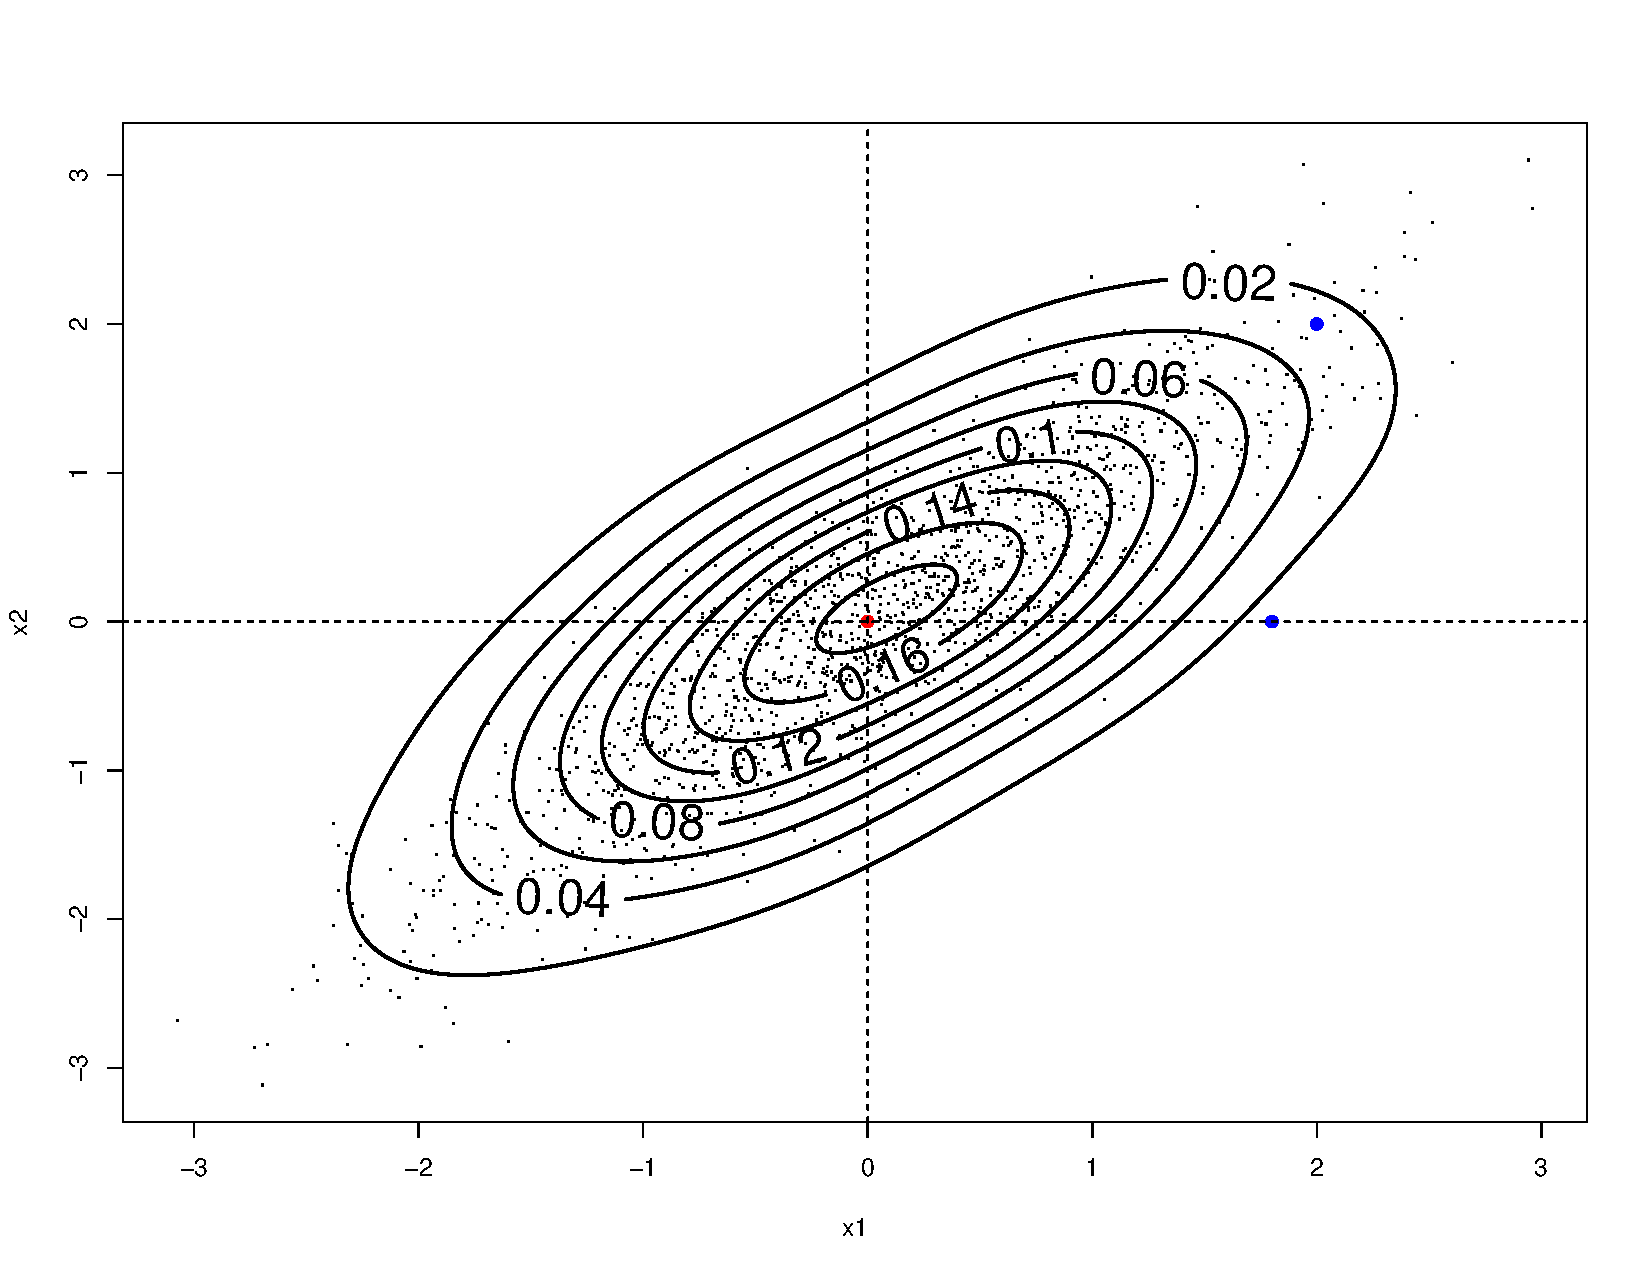
\includegraphics[height=.35\textheight]{Maha1.pdf}\end{center}
\onslide<4-> \textbf{Others:} coarsened exact matching, genetic matching, \ldots
\end{frame}


% \begin{frame}{Distance metrics (II): coarsened and learned}
% \small
% \onslide<1-> \textbf{Coarsened Exact Matching (CEM):} bin each covariate coarsely, match exactly within bins. \\
% Exact within bin; discards units without a bin-mate (transparent off-support cost).

% \medskip
% \onslide<2-> \textbf{Genetic matching:} search covariate weights $W$ in\\[2pt]
% $d(X_i,X_j) = \sqrt{(X_i{-}X_j)' \widehat{\Sigma}_X^{-1/2}\,W\,\widehat{\Sigma}_X^{-1/2}(X_i{-}X_j)}$\\[2pt]
% that maximise post-match balance (Diamond \& Sekhon 2013).

% \medskip
% \onslide<3-> \textbf{Propensity-score distance:} $d = |\widehat\pi(X_i) - \widehat\pi(X_j)|$ --- collapses $X$ to a scalar. (\S3.)
% \end{frame}


\begin{frame}{Matching routines}
\footnotesize
\onslide<1-> \textbf{1-to-1 vs 1-to-M.} Match each treated to one control, or to $M$ nearest (then average). Larger $M$: lower variance, higher bias.

\medskip
\onslide<2-> \textbf{With vs without replacement.}
\begin{itemize}\itemsep1pt
\item \textit{With}: a control may match many treated. Lower bias, higher variance.
\item \textit{Without}: each control used once, can force bad matches when $n_0$ small.
\end{itemize}

\medskip
\onslide<3-> \textbf{Greedy vs optimal.}
\begin{itemize}\itemsep1pt
\item \textit{Greedy}: step through treated units, grab nearest available control.
\item \textit{Optimal}: minimise \textit{total} within-pair distance across the whole match.
\end{itemize}

\medskip
\onslide<4-> \textbf{Full / complete matching} (Hansen 2004): every treated matched to $\geq 1$ control \textit{and} vice versa; variable-size sets. Uses all data.

\end{frame}


\begin{frame}{Limits of matching (I): discrepancy}
\small
\onslide<1-> Matched pairs are never exactly equal in $X$ (except under exact match). Discrepancy $\|X_i - X_{j(i)}\|$ leaves residual bias on each pair.

\medskip
\onslide<2-> \textbf{Abadie \& Imbens (2006):} matching bias does not shrink at $\sqrt{n}$ once $\dim(X) \geq 2$ with continuous $X$. Matching alone is not $\sqrt{n}$-consistent.

\medskip
\onslide<3-> \textbf{Bias-adjusted matching:} fit $\widehat{\mu}_0(X)$ among controls, replace $Y_{j(i)}$ with $Y_{j(i)} - [\widehat{\mu}_0(X_{j(i)}) - \widehat{\mu}_0(X_i)]$. A ``little regression'' fills the gap.

\end{frame}


\begin{frame}{Limits of matching (II): curse of dimensionality}
\footnotesize
\onslide<1-> As $\dim(X)$ grows, everyone is far away. %With $X$ uniform on $\mathbb{R}^P$, Euclidean radius $r$ for a ball to contain 1\% of mass:
\begin{center}
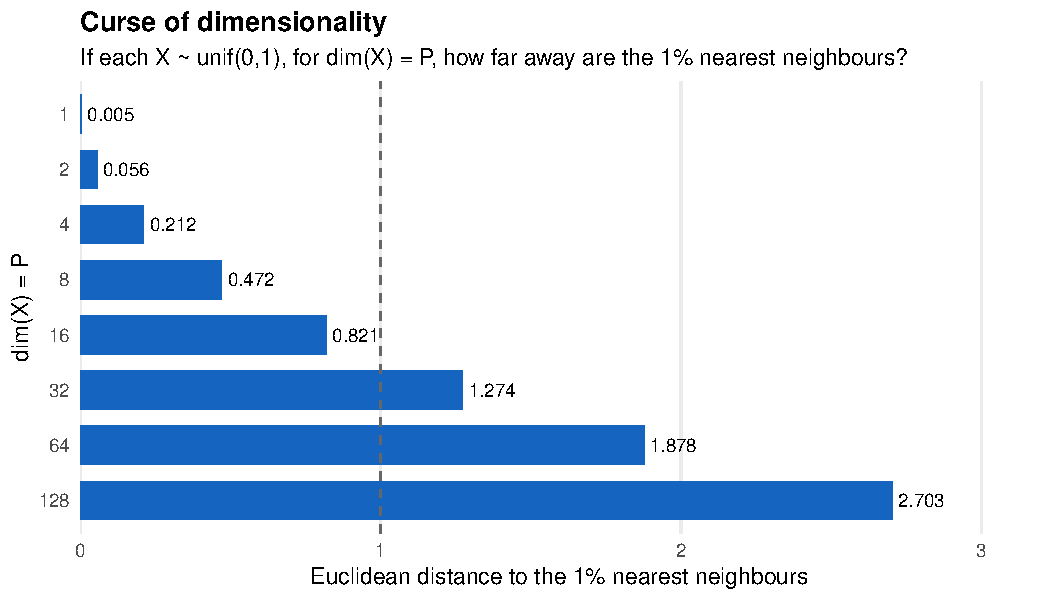
\includegraphics[width=.72\textwidth]{curse_of_dim.pdf}
\end{center}
Broader point: Matching is appealingly nonparametric, but you pay a price in bias, especially as $P$ grows.
\end{frame}


%% =====================================================================
\section{Propensity score: a dimension reducer}
%% =====================================================================

\begin{frame}{Propensity score}
\small
\onslide<1-> Define $\pi(X) := \Pr(D = 1 \mid X)$.

\medskip
\onslide<2-> \textbf{Rosenbaum \& Rubin (1983).} If $\{Y_1, Y_0\} \indep D \mid X$, then $\{Y_1, Y_0\} \indep D \mid \pi(X)$.

\medskip
\onslide<3-> Why it matters: a scalar summary of $X$ is enough to achieve CI. \\

\medskip
\onslide<4-> Two families of use:
\begin{itemize}
\item \textbf{PS matching / stratification}: match or stratify on $\widehat\pi(X)$.
\item \textbf{IPW}: reweight by $1/\widehat\pi(X)$ (next section).
\end{itemize}

\medskip
\onslide<5-> Costs:
\begin{itemize}
\item You have to specify a model for $\pi(X)$, if wrong, $\hat{\tau}$ inconsistent.
\item You don't get ``exact balance'' on $X$ in any sense.
\end{itemize}
\end{frame}


\begin{frame}{PS matching:}
\small
\onslide<1-> First idea: match treated $i$ to control $j$ minimizing $|\widehat\pi(X_i) - \widehat\pi(X_j)|$.\\
\medskip
\onslide<2-> Let's see what $\hat{\pi}(X)$ looks like in LaLonde (logit model)
\medskip
\onslide<2-> \begin{center}
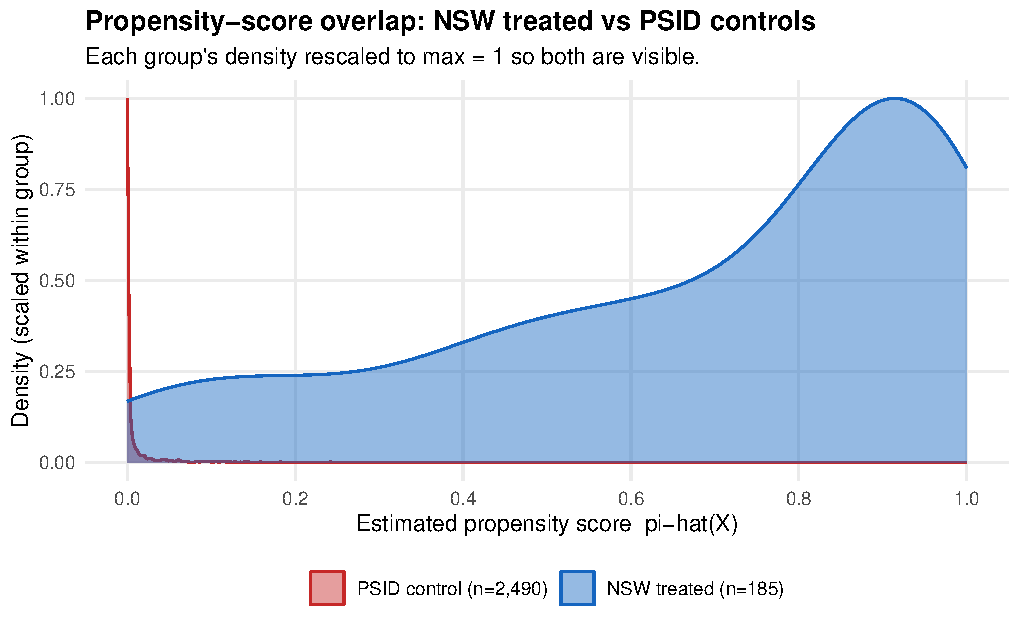
\includegraphics[width=.95\textwidth]{lalonde_pscore.pdf}
\end{center}

\onslide<3-> Here the smart play is: only ask about ATT.\\
\medskip
\onslide<4-> If two-sided poor overlap, you wouldn't be able to do anything. 
\end{frame}


%% =====================================================================
\section{Inverse-propensity weighting}
%% =====================================================================

\begin{frame}{IPW: reweighting to the target distribution}
\small
\onslide<1-> Matching suffers discrepancies and throws away observations--- just weight!\\
\footnotesize
\begin{itemize}
\item<2-> Treated arm has covariate density $p(X\mid D{=}1)$; we want $p(X)$.
\item<3-> Multiply each treated unit by $p(X)/p(X\mid D{=}1)$ to match $p(X)$.
\item<4-> But $p(X \mid D=1)$ is poorly estimated, so rewrite  $p(X)/p(X\mid D{=}1) = p(D=1)/p(D=1\mid X) = p(D=1)/\pi(X)$.
\item<5-> Likewise for controls, weight by $p(D=0)/(1-\pi(X))$.
\end{itemize}
\medskip
\small
\onslide<4-> These are the (\textbf{stabilised}) IPW weights:
\scriptsize
\[ w_i = \frac{D\,\Pr(D{=}1)}{\widehat\pi(X_i)} + \frac{(1-D)\,\Pr(D{=}0)}{1-\widehat\pi(X_i)} \]
\medskip
\small
\onslide<5-> Use them to weight the DIM for the ATE:
\scriptsize
$$\widehat\tau_{\text{IPW}} \;=\; \frac{\sum_i w_i D_i Y_i}{\sum_i w_i D_i} \;-\; \frac{\sum_i w_i (1-D_i) Y_i}{\sum_i w_i (1-D_i)}.$$
\small
\onslide<6-> \textbf{ATT version}: treated $w_i = 1$ (already at target); controls $w_i = \dfrac{\widehat\pi(X_i)}{1-\widehat\pi(X_i)}\cdot\dfrac{\Pr(D{=}0)}{\Pr(D{=}1)}$ (Bayes for $p(X\mid D{=}1)/p(X\mid D{=}0)$).
\end{frame}


\begin{frame}{Worry about the weights}
\footnotesize
\onslide<1-> Weights blow up when $\widehat\pi \to 0$ (treated) or $\to 1$ (controls). \\
\medskip
\onslide<2-> The few treated units that look PSID-like (low $\widehat\pi$) get astronomical weights:
\begin{center}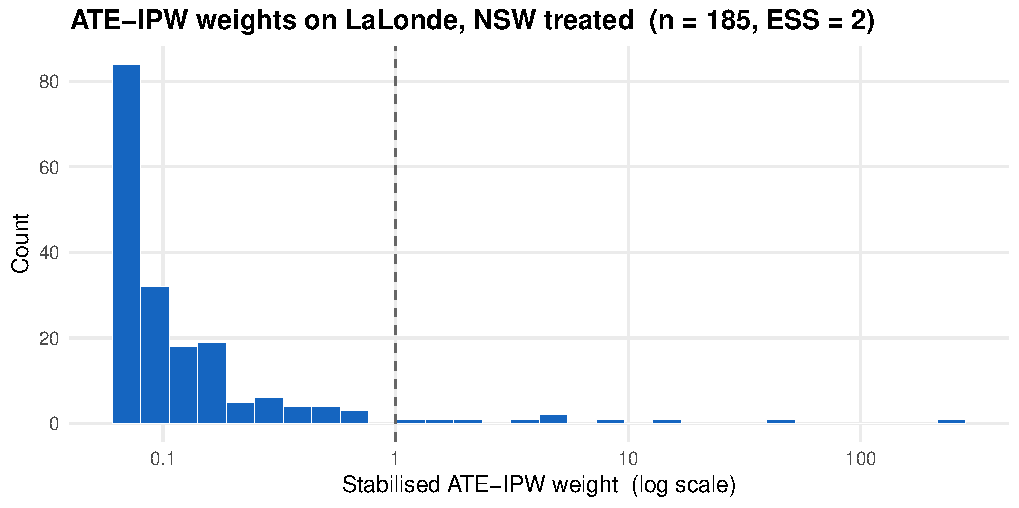
\includegraphics[width=.7\textwidth]{lalonde_ipw_weights.pdf}\end{center}
\begin{itemize}
\item<3-> One treated unit gets a weight over 240, carrying 70\% of the treated weight;
\item<4-> For treated, ESS $= (\sum w_i)^2 / \sum w_i^2 \approx 2!$ (from 185).
\item<5-> For controls, many get downweighted but ESS $\approx$ 711 (from 2490). ATT fine.
\end{itemize}
\end{frame}


%% =====================================================================
\section{Balancing weights}
%% =====================================================================

\begin{frame}{Balancing weights: solve directly}
\small
\onslide<1-> If you want $p(X\mid D=1) \approx p(X \mid D=0)$, why not just choose weights $\{w_i\}$ s.t. weighted control distribution matches treated (ATT) or target (ATE) on (chosen moments of) $X$? \\
\medskip
\onslide<2-> \textbf{Mean-balance constraint} (in ATT case):
$$\sum_{i:\, D_i=1} \phi(X_i) \;=\; \sum_{i:\, D_i=0} w_i\, \phi(X_i), \quad \text{s.t.}\;\sum w_i = n_1, \quad w_i \geq 0 \;\forall i$$
\noindent for some map $\phi(X)$ (e.g.\ $\phi(X)=X$ for mean balance; $\phi(X)=K(X,\cdot)$ for kernel balance).\\
\medskip
\onslide<3-> Constraint alone is under-determined. Add a regulariser on $w$ such as:
\begin{itemize}
\item Maximum entropy: $\min \sum_i w_i \log w_i$ $\rightarrow$ entropy balancing (Hainmueller 2012)
\item $L_2$ penalty: $\min \sum_i w_i^2$ $\rightarrow$ stable balancing weights (Zubizarreta 2015)
\item Empirical likelihood, $\sum_i log(w_i)$
\end{itemize}
\end{frame}

\begin{frame}{Balance on LaLonde: unweighted vs IPW vs ebal}
\small
\vspace{-0.3em}
Standardised mean differences across covariates: unweighted is far off; IPW shrinks the gap but \textit{doesn't} hit zero (and can still miss); entropy balancing zeroes the means by construction.
\begin{center}
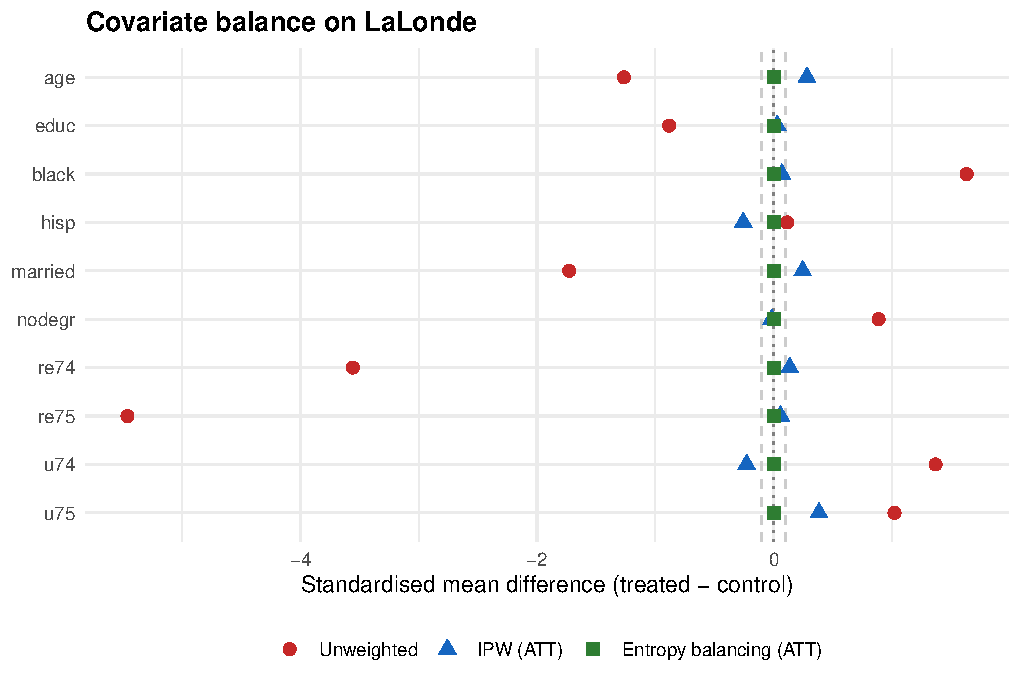
\includegraphics[width=.74\textwidth]{lalonde_balance.pdf}
\end{center}
\end{frame}

\begin{frame}{CBPS (Imai \& Ratkovic 2014): a pscore tuned for balance}
\small
\onslide<1-> What if we still want a pscore (interpretable, parametric, easy to inspect) but tune it so the resulting IPW gives exact finite-sample balance? Stack the moment conditions per unit:
$$\phi(X_i, D_i;\beta) \;=\; \begin{pmatrix}
\bigl[D_i - \pi(X_i;\beta)\bigr]\, X_i \\[6pt]
\left[\dfrac{D_i}{\pi(X_i;\beta)} - \dfrac{1-D_i}{1-\pi(X_i;\beta)}\right]\, X_i
\end{pmatrix}.$$
{\footnotesize Top: standard logistic MLE score (what logistic regression solves). Bottom: IPW balance moment --- forces IPW-reweighted means of $X$ to match across arms.}

\medskip
\onslide<2-> Choose $\beta$ to set the moments to zero:
\begin{itemize}\itemsep1pt
\item \textbf{M-estimator} (just-identified): keep $k$ of the $2k$ moments --- e.g.\ balance only --- and solve $\sum_i \phi^{(j)}(X_i;\beta) = 0$.
\item \textbf{GMM} (over-identified, both rows): $\widehat\beta = \arg\min_\beta \bigl[\tfrac{1}{n}\sum_i \phi\bigr]'\,W\,\bigl[\tfrac{1}{n}\sum_i \phi\bigr]$.
\end{itemize}
\end{frame}



\begin{frame}{Beyond means; prognostic balancing}
\small
\onslide<1-> \textbf{What does mean balance buy?} Choosing $\phi(X) = X$ balances $X$'s means across arms --- which translates into balance on \textit{linear functions} of $X$.
\begin{itemize}\itemsep1pt
\item If $\mu_0(X)$ is linear in $X$, that's exactly what you need: $\E[\mu_0(X)]$ matches across arms and $\widehat\tau$ is unbiased.
\item If $\mu_0(X)$ has nonlinearities or interactions, mean-balanced $X$ does \emph{not} imply balanced $\mu_0(X)$. Residual bias remains.
\end{itemize}

\medskip
\onslide<2-> \textbf{Prognostic balancing} (for ATT): what we really want is $\E[\mu_0(X)]$ equal across arms. Balance directly on $\widehat\mu_0(X)$, the prognostic score.
\begin{itemize}\itemsep1pt
\item Fit $\widehat\mu_0(X)$ on controls; project onto all units.
\item Solve for control weights so $\sum_{i:D=0} w_i \widehat\mu_0(X_i) = \sum_{i:D=1} \widehat\mu_0(X_i)$.
\item $\widehat\mu_0$ can be OLS, ML, anything. Flexibility propagates into the weights.
\end{itemize}

\medskip
\onslide<3-> \textcolor{Blue}{Efficient; handy especially when poor overlap on (non-prognostic) $X$. Work in progress.}
\end{frame}

% \begin{frame}{Balancing: what it buys and what it costs}
% \small
% \onslide<1-> \textbf{Buys:} in-sample exact balance on whatever you target; no need to specify $\pi$.

% \medskip
% \onslide<2-> \textbf{Costs:}
% \begin{itemize}
% \item You only balance on what you include. Unmodelled nonlinearities or interactions still confound.
% \item Weights can be extreme if no good balancing solution exists --- a symptom of poor overlap.
% \end{itemize}
% \end{frame}





%% =====================================================================
\section{Regression, via imputation}
%% =====================================================================

\begin{frame}{G-computation / imputation}
\small
\onslide<1-> Instead of weighting, \textit{model} $\mu_1(x)$ and $\mu_0(x)$. Then impute each unit's missing potential outcome:
$$\widehat{\tau} \;=\; \frac{1}{n}\sum_{i=1}^n\!\left[\widehat{\mu}_1(X_i) - \widehat{\mu}_0(X_i)\right].$$

\medskip
\onslide<2-> Fit $\widehat{\mu}_1$ on treated only, $\widehat{\mu}_0$ on controls only (\textbf{T-learner}).

\medskip
\onslide<3-> For ATE, average over all $X_i$; for ATT, over treated $X_i$; for ATC, over controls.

\medskip
\onslide<4-> Functional form of $\widehat\mu_d$ is your choice: OLS, random forest, kernel regression, \ldots
\end{frame}


% \begin{frame}{Pooled OLS gets it wrong in general}
% \small
% \onslide<1-> \textbf{Pooled, no interaction:} $Y = \alpha + \tau D + \beta' X + \varepsilon$.

% \medskip
% \onslide<2-> This forces a \textit{common} slope in $X$ for treated and control.

% \medskip
% \onslide<3-> Under effect heterogeneity $\mu_1(X) - \mu_0(X)$ varying in $X$, the fitted $\widehat\tau$ is a weighted combination of unit-level effects --- weights determined by residual variation in $D$ given $X$. Not the ATE, not the ATT.

% \medskip
% \onslide<4-> The fix: let the slope differ by $D$. That gives us Lin's estimator.
% \end{frame}


\begin{frame}{Lin's estimator (interacted OLS)}
\small
\onslide<1-> \textbf{Lin (2013).} Fit the fully interacted model
$$Y \;=\; \alpha + \tau D + \beta' X + \gamma'(X \cdot D) + \varepsilon.$$

\medskip
\onslide<2-> Equivalent to fitting two separate OLS models ($\widehat{\mu}_1$ on treated, $\widehat{\mu}_0$ on controls) and reading off $\widehat\mu_d(x) = \widehat\alpha_d + \widehat\beta_d' x$.

\medskip
\onslide<3-> \textbf{Two things to want from this regression.}
\begin{itemize}
\item The coefficient on $D$ should be the \textit{average} treatment effect, not ``effect at $X=0$.''
\item The coefficient should equal the g-computation imputation estimate $\tfrac{1}{n}\sum_i[\widehat{\mu}_1(X_i) - \widehat{\mu}_0(X_i)]$.
\end{itemize}

\medskip
\onslide<4-> \textcolor{Blue}{We get both if we center $X$ first.}
\end{frame}


\begin{frame}{Centering $X$: why and what it buys}
\small
\onslide<1-> Let $\tilde X_i = X_i - \bar X$ (sample-mean-centred). The interacted model becomes
$$Y \;=\; \alpha + \tau D + \beta' \tilde X + \gamma'(\tilde X \cdot D) + \varepsilon.$$

\medskip
\onslide<2-> Unit-level treatment effect at $X = x$:
$$\partial Y / \partial D \;=\; \tau + \gamma'\tilde X \;=\; \tau + \gamma'(x - \bar X).$$

\medskip
\onslide<3-> \textbf{(i) Average effect.}
$$\frac{1}{n}\sum_{i=1}^n \partial Y_i / \partial D
\;=\; \tau + \gamma' \underbrace{\tfrac{1}{n}\sum_i(X_i - \bar X)}_{=\,0}
\;=\; \tau.$$

% \medskip
% \onslide<4-> \textbf{(ii) Effect at the mean.} Evaluate $\partial Y/\partial D$ at $x = \bar X$: $\tilde X = 0$, so $\partial Y/\partial D = \tau$.

% \medskip
% \onslide<5-> \textcolor{Blue}{Mean of the unit-level slope $\;=\;$ slope at the mean $\;=\;$ the coefficient $\widehat\tau$ on $D$.}

% \medskip
% \onslide<6-> Same holds for the imputation average (next frame).
\end{frame}


\begin{frame}{And the (linear) imputation estimator does just that:}
\small
\onslide<1-> Fitted means:
\begin{align*}
\widehat{\mu}_1(x) &= \widehat\alpha + \widehat\tau + \widehat\beta'(x - \bar X) + \widehat\gamma'(x - \bar X) \\
\widehat{\mu}_0(x) &= \widehat\alpha + \widehat\beta'(x - \bar X)
\end{align*}

\medskip
\onslide<2-> Imputation (g-comp) estimate:
$$\frac{1}{n}\sum_{i=1}^n \left[\widehat{\mu}_1(X_i) - \widehat{\mu}_0(X_i)\right]
\;=\; \widehat\tau + \widehat\gamma'\underbrace{\tfrac{1}{n}\sum_i (X_i - \bar X)}_{=\,0}
\;=\; \widehat\tau.$$

\medskip
\onslide<3-> So with centered $X$, three things collapse to one number:
\begin{itemize}\itemsep1pt
\item the coefficient $\widehat\tau$ on $D$,
\item the average unit-level slope,
\item the g-computation / T-learner imputation estimate.
\end{itemize}
\end{frame}


% \begin{frame}{Lin: SEs and where this lands us}
% \small
% \onslide<1-> \textbf{SEs.} Use HC2 (or cluster-robust analogue). Lin (2013) shows: under arbitrary effect heterogeneity, interacted OLS is consistent \textit{and} its robust SE is asymptotically valid.
% \onslide<2-> No worse than un-interacted OLS under homogeneity --- and right in general.

% \medskip
% \onslide<3-> Connection to Unit 2: this is the observational analogue of the Lin-adjusted experimental estimator we used for precision improvement.

% \medskip
% \onslide<4-> \textbf{Rules of thumb.}
% \begin{itemize}
% \item Always centre covariates before interacting with $D$.
% \item Read $\widehat\tau$ as ATE when centred at $\bar X$; ATT when centred at $\bar X_1$; ATC at $\bar X_0$.
% \item Use HC2 (or CR2 with clusters).
% \end{itemize}
% \end{frame}


%% =====================================================================
\section{All roads lead to the same place}
%% =====================================================================

\begin{frame}{All roads lead to the same place}
\small
\onslide<1-> Under CI, every method is estimating $\E_{X\sim F}[\mu_1(X) - \mu_0(X)]$.

\medskip
\onslide<2->
\begin{center}
\renewcommand{\arraystretch}{1.25}
\begin{tabular}{ll}
\toprule
\textbf{Method} & \textbf{How it approximates conditioning on $X$} \\
\midrule
Subclassification & coarse strata of $X$ \\
Matching          & nearest-neighbour ``strata of one'' in $X$ \\
PS matching       & match on scalar $\pi(X)$ \\
IPW               & reweight by $1/\pi(X)$ \\
CBPS              & estimate $\pi$ s.t.\ balance constraint holds \\
Balancing weights & solve for weights balancing $X$ (or $\phi(X)$) \\
Kernel balancing (kbal) & balance on a basis expansion of $X$ \\
Prognostic balancing & balance on $\widehat\mu_0(X)$ \\
Regression imputation & model $\mu_d(X)$ (Lin); impute \\
\bottomrule
\end{tabular}
\end{center}

\medskip
\onslide<3-> \textcolor{Blue}{One angle: Choose the appropriate set of these for your problem, and implement them all. If they disagree, diagnose.}
\end{frame}


\begin{frame}{LaLonde: tough one due to overlap}
\vspace{-0.5em}
\begin{center}
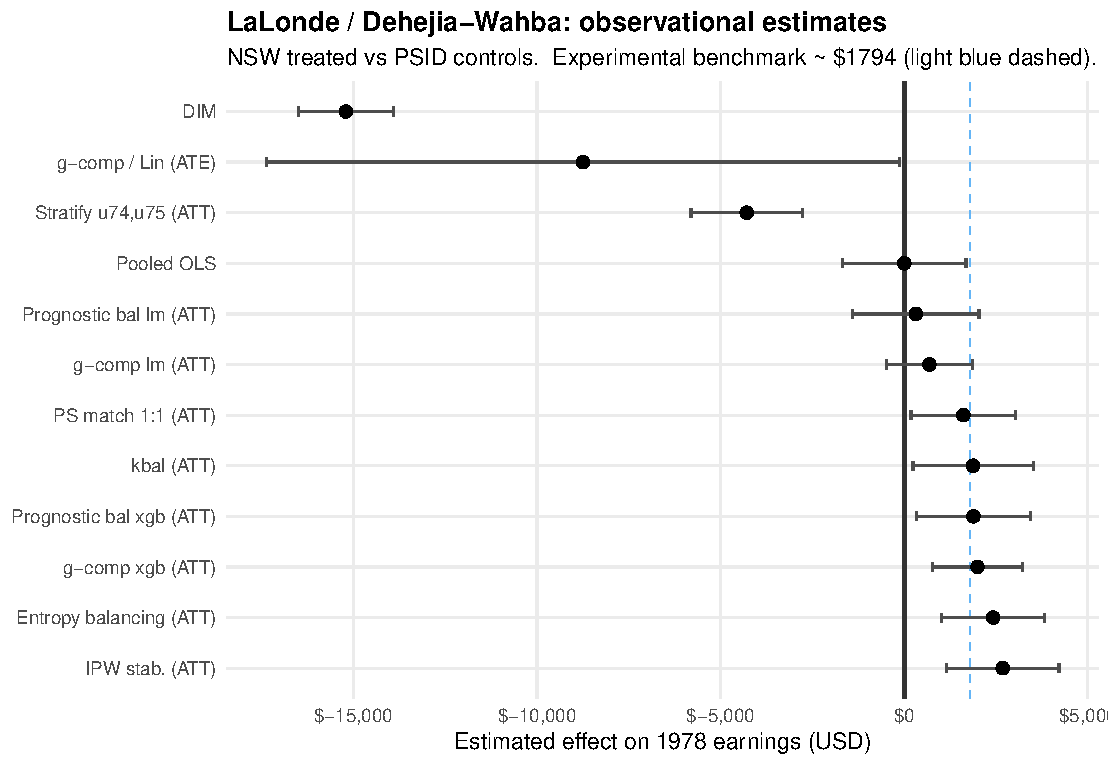
\includegraphics[width=.92\textwidth]{lalonde_estimates.pdf}
\end{center}
\end{frame}


\begin{frame}{Lessons from LaLonde}
\small
\onslide<1-> \textbf{ATE on LaLonde is a trap.} Two faces of the same issue:\\
\begin{itemize}
\item<2-> g-comp / Lin (ATE) lands at $-\$8{,}746$: $\widehat\mu_1(X)$ must be extrapolated to 2,490 PSID-like $X$'s where no treated unit lives. Huge variance ensues.
\item<3-> IPW (ATE) fails because the rare \textit{treated} units that look PSID-like get huge weights\,---\,effective treated $N$ collapses from 185 to $\approx 2$.
\end{itemize}

\medskip
\onslide<4-> \textbf{Retreat to ATT.} The treated do have controls around them, so ATT is fine. 
\begin{itemize}
\item<5-> But if you need to learn $\mu_0(X)$, learn it in a way that can specialise local structure since many controls are far from treated.
\end{itemize}
% \begin{frame}{Lessons from LaLonde (II): outcome model}
% \small
% \onslide<1-> \textbf{Global vs local learning of $\widehat\mu_0$ matters.} \\
% Linear $\widehat\mu_0$ is fit on the 2{,}490 PSID mass and applied to 185 NSW-like $X$'s --- a rule learned from distant data. Tree-based $\widehat\mu_0$ (xgb) partitions $X$ and predicts near the treated region from \textit{nearby} controls. This hurts methods that rely on $\widehat\mu_0$:
% \begin{itemize}\itemsep1pt
% \item g-comp (ATT): \$688 $\to$ \$1{,}998
% \item prognostic balancing (ATT): \$320 $\to$ \$1{,}887
% \end{itemize}

\medskip
\onslide<6-> \textbf{The ATT cluster near \$1{,}794.} PS match, IPW, entropy balancing, kbal, g-comp xgb, and prognostic balancing with xgb all land close to the benchmark. When covariate shift is severe, reweighting or locally-adaptive imputation works well.
\medskip
\onslide<7-> \textcolor{Blue}{General rule: choose the estimand and the family of estimators for your situation.}
\end{frame}


\begin{frame}{Augmented / doubly robust: a signpost}
\small
\onslide<1-> Methods that use \textbf{both} $\widehat\pi$ and $\widehat{\mu}_d$:
\begin{itemize}
\item \textbf{AIPW}: IPW estimator plus a regression adjustment (equivalently, g-comp plus IPW-weighted residuals). Consistent if \textit{either} $\widehat\pi$ or $\widehat\mu_d$ is right.
\item \textbf{TMLE}: iteratively tilt $\widehat\mu_d$ using $\widehat\pi$ to solve an efficient score equation.
\item \textbf{DML} (Chernozhukov et al.\ 2018): put flexible ML $\widehat\pi,\widehat\mu_d$ together with \textit{cross-fitting}. Delivers $\sqrt{n}$-valid inference despite ML bias.
\end{itemize}

\medskip
\onslide<2-> These are candidates for the Advanced Topic Presentation: ``efficiency and flexibility in covariate adjustment.''

\medskip
\onslide<3-> \textcolor{Blue}{If nobody picks it, I might carve out a lecture.}
\end{frame}

% %% =====================================================================
% \section{Falsification}
% %% =====================================================================

% \begin{frame}{Placebo / falsification checks}
% \small
% \onslide<1-> All of the above assume CI. Can we check it? Strictly no. But we can falsify it.

% \medskip
% \onslide<2-> Three standard placebos:
% \begin{itemize}
% \item \textbf{Placebo outcome}: an outcome that \textit{should not} respond to $D$. If your adjustment strategy finds a non-zero effect there, something's wrong.
% \item \textbf{Placebo treatment}: a sham treatment that wasn't actually administered. Same logic.
% \item \textbf{Placebo group / differencing group}: a population that shouldn't be affected.
% \end{itemize}

% \medskip
% \onslide<3-> Balance tests are a special case: you check that $X$ is balanced post-adjustment. \textit{But balance on observed $X$ says nothing about unobserved $U$.}

% \medskip
% \onslide<4-> \textcolor{Blue}{Placebos can falsify, never confirm. If they \textit{reject}, believe it. If they don't, keep worrying.}
% \end{frame}


%% =====================================================================
\section{Close}
%% =====================================================================

\begin{frame}{Takeaways}
\small
\onslide<1-> \textbf{One target.} Under CI, everything estimates $\E_{X\sim F}[\mu_1(X) - \mu_0(X)]$. Choose $F$ for the estimand; choose a method for how to approximate conditioning on $X$.

\medskip
\onslide<2-> \textbf{Method menu.} Subclass / matching / PS-matching / IPW / balancing weights / regression imputation (Lin). Pick based on what you're willing to model.

\medskip
\onslide<3-> \textbf{Lin}: interacted OLS on \textit{centered} $X$ gives a $D$-coefficient equal to the g-computation estimate. Center at the right mean for your estimand.

\medskip
\onslide<4-> \textbf{Extrapolation is not reweighting.} On LaLonde, OLS-ATE extrapolates $\widehat\mu_1$ far outside the treated support and lands at $-\$8{,}746$; the ATT version is $+\$688$; weighting methods cluster near the truth. \textit{Pick estimand and method with an eye on support.}

\medskip
\onslide<5-> \textbf{What's still missing.} Unobserved confounding. When CI fails, every method on this menu is biased.
\end{frame}


\end{document}
